
%(BEGIN_QUESTION)
% Copyright 2011, Tony R. Kuphaldt, released under the Creative Commons Attribution License (v 1.0)
% This means you may do almost anything with this work of mine, so long as you give me proper credit

The following FOUNDATION Fieldbus control loop uses three redundant temperature transmitters (each one measuring temperature at the same physical location in the process) to control one valve.  This diagram shows the interconnections of all function blocks, as well as the instrument locations of each block (in italics):

$$\includegraphics[width=15.5cm]{i03643x01.eps}$$

Suppose the control system is working perfectly, with all three transmitters reporting the same temperature (380 degrees F) which is also equal to setpoint.  Determine the system's immediate response in these two scenarios, considered one at a time:

\vskip 10pt

\begin{itemize}
\item{} TT\_102a's sensor fails so that it transmits a 70 degree F signal with ``Good'' status
\vskip 20pt
\item{} TT\_102b fails so that it stops communicating on the Fieldbus segment
\vskip 20pt
\end{itemize}

\underbar{file i03643}
%(END_QUESTION)





%(BEGIN_ANSWER)

\begin{itemize}
\item{} TT\_102a's sensor fails: {\it PV signal to PID block becomes 276.7 degrees F; valve takes action to raise PV back to 380 degrees.}
\item{} TT\_102b stops communicating: {\it PID block senses lack of input signal and sheds to a safe operating mode (most likely ``Initialization Manual'').}
\end{itemize}

%(END_ANSWER)





%(BEGIN_NOTES)

{\bf This question is intended for exams only and not worksheets!}.

%(END_NOTES)


